%------------------------------------------------------------
% DEFINITIONS AND HEADERS -- IGNORE THIS
%------------------------------------------------------------
\documentclass{article}
\usepackage[top=2.2cm, bottom=2.1cm, left=2.2cm, right=2.2cm]{geometry}
\usepackage[utf8]{inputenc}
\usepackage{algpseudocode}
% Get better typography
\usepackage[protrusion=true,expansion=true]{microtype}  
% For algorithms
\usepackage[boxruled,linesnumbered,vlined,inoutnumbered]{algorithm2e}
\SetKwInOut{Parameter}{Parameters}
% For basic math, align, fonts, etc.
\usepackage{amsmath}
\usepackage{amsthm}
\usepackage{amssymb}
\usepackage{mathtools}
\usepackage{mathrsfs}
\usepackage{rotating}
\usepackage{tabularx}
\usepackage{booktabs}
\usepackage{soul}
\usepackage{changepage}
\usepackage{gensymb} % For \degree
\usepackage{lscape}
% For \thead to make line breaks in tables
\usepackage{array}
\usepackage{makecell}
\renewcommand\theadalign{bc}
\renewcommand\theadfont{\bfseries}
\renewcommand\theadgape{\Gape[4pt]}
\renewcommand\cellgape{\Gape[4pt]}
\usepackage{courier} % For \texttt{foo} to put foo in Courier (for code / variables)
\usepackage{lipsum} % For dummy text
% For images
\usepackage{graphicx}
\usepackage{subcaption}
\usepackage[space]{grffile} % For spaces in image names
\usepackage{float}
\usepackage{fancyvrb}
% For bibliography
\usepackage[round]{natbib}
% For color
\usepackage{xcolor}
\definecolor{light-grey}{rgb}{0.9,0.9,0.9}
\definecolor{dark-red}{rgb}{0.4,0.15,0.15}
\definecolor{dark-blue}{rgb}{0,0,0.7}
\definecolor{darkblue}{rgb}{0,0,.6}
\definecolor{darkred}{rgb}{.58,0,0}
\definecolor{brighterred}{rgb}{.745,0,0}
\definecolor{darkgreen}{rgb}{0,.6,0}
\definecolor{red}{rgb}{.98,0,0}
\usepackage{environ}
% Only show sections in table of contents and rename
\setcounter{tocdepth}{2}
\renewcommand{\contentsname}{Table of Contents}
% For links (e.g., clicking a reference takes you to the phy)
\usepackage{hyperref}
\hypersetup{
    colorlinks, linkcolor={dark-blue},
    citecolor={dark-blue}, urlcolor={dark-blue}
}
\newcommand{\HIGHLIGHT}[1]{\textcolor{blue}{\textbf{#1}}}
% \newcommand{\Solution}[1]{{\color{blue} \paragraph{\bf $\bigstar $ SOLUTION:} { \sf
%     #1} \bigskip}}
\newcommand{\TODO}[1]{\textcolor{blue}{\textbf{{#1}}}}
\newcommand{\POINTS}[1]{\textcolor{purple}{\textbf{{#1}}}}
\providecommand{\mathcolor}[2]{\textcolor{#1}{#2}}
% My definition of "summary boxes" (see below)
\usepackage[most]{tcolorbox}
\definecolor{boxgray}{rgb}{0.95, 0.95, 0.95}
\definecolor{boxblue}{rgb}{0.941, 0.941, 0.98}
\definecolor{boxpink}{rgb}{1.0, 0.93, 0.93}
\definecolor{boxwhite}{rgb}{1.0, 1.0, 1.0}
%\definecolor{boxgreen}{rgb}{0.91, 0.96, 0.9}
\definecolor{boxgreen}{rgb}{0.92, 0.96, 0.92}
\newtcolorbox{mybox}[1][boxwhite]{%
  enhanced,
  boxrule=0.5pt,
  colframe=black,
  colback=#1,
  sharp corners,
  width=\linewidth,
  left=1em,
  right=1em,
  top=0.5em,
  bottom=0.5em,
  boxsep=0pt,
  before skip=1em,
  after skip=0.85em,
}
%------------------------------------------------------------





\usepackage{colortbl}

\begin{document}
\vspace*{1cm}
\begin{center}
    \begin{Large}
    COMPSCI 589 Final Project - Fall 2026
    \end{Large}
    \\
    \vspace{0.15cm}
    Due \textcolor{darkred}{\textbf{December 15}}, 11:55 pm Eastern Time
    \\[0.35cm]
    \textbf{Group: Hoa La, \textcolor{red}{[Teammate 2]}, \textcolor{red}{[Teammate 3]}}
\end{center}

\vspace{0.5cm}
\section*{How to run code}

Python 3 with numpy and matplotlib. scikit-learn is only used to load the Digits dataset
(datasets.load\_digits, as in the handout). From the code/ folder:

\begin{verbatim}
pip install -r requirements.txt
python run_experiments.py               # all 5 datasets (4 + CMC)
python run_experiments.py digits rice   # or only some of them
\end{verbatim}

The three csv files go in code/, code/data/, or the supporting files folder next to code/. Every number
and graph in this report is written to code/output/ (one results\_<dataset>.json per dataset). Seed 589.

\begin{itemize}
\item knn.py: $k$-NN (Hoa La, HW1).
\item decision\_tree.py, random\_forest.py: decision tree and random forest (Hoa La, HW1 and HW3).
\item neural\_net.py: neural network with backpropagation (Hoa La, HW4). Only change: with more than one
output neuron, predict returns the class of the largest output (needed for Digits).
\item extra\_trees.py: extra trees, new for extra credit 4 (Hoa La), built on the HW3 tree code.
\item data/cmc.csv: the extra dataset for extra credit 2, converted from UCI to the same csv format.
\item utils.py: loading, one-hot encoding, normalization, stratified folds, metrics.
\item run\_experiments.py, plotting.py: all experiments and graphs.
\end{itemize}

\section*{Setup}

\textbf{Implementations.} All three algorithms use Hoa La's code from the homeworks.

\textbf{Algorithms.} We ran $k$-NN, random forest and neural network on every dataset
(three algorithms, so this is also extra credit 1). They cover the three kinds of model from the course:
$k$-NN compares instances by distance, the random forest splits on one attribute at a time and averages
many trees, and the neural network learns a smooth boundary over all inputs at once. Each dataset section
says why we expected each one to work there.

\textbf{Evaluation.} Stratified 10-fold cross-validation (the HW3 folds). All algorithms on a dataset use
the same 10 folds, so they are compared on exactly the same splits. Accuracy and F1 are averaged over
the 10 test folds. F1 uses one positive class per binary dataset (named below). Digits has 10 classes, so
we report macro-F1: the F1 of each digit as the positive class, averaged over the 10 digits.

\textbf{Preprocessing.} The random forest uses categorical attributes directly (one child per value,
as in HW3). For $k$-NN and the neural network, categorical attributes are one-hot encoded, and all
inputs are min-max normalized using the training folds only.

\textbf{Hyperparameters.} Chosen by F1 in the same 10-fold CV, like in HW3 and HW4.
\begin{itemize}
\item $k$-NN: 10 values of $k$, from 1 to 51.
\item Random forest: 6 stopping criteria at $ntree = 10$, then $ntree \in \{1, 5, 10, 20, 30, 40, 50\}$ with the best one.
$m = \sqrt{\#\text{attributes}}$ attributes per split, numerical splits at the mean (HW3).
\item Neural network: first $\alpha \in \{0.3, 1, 3\}$ and $m \in \{100, 300\}$ epochs on one hidden layer of
16 with $\lambda = 0$ (stopping criterion: fixed $m$ epochs). Then 6 architectures $\times$
$\lambda \in \{0, 0.1, 1\}$ = 18 networks. Mini-batch 32, sigmoid units, one output neuron for binary
datasets and 10 (one per digit) for Digits.
\end{itemize}

\textbf{Graphs.} Same as the homeworks: performance vs.\ $k$ for $k$-NN, performance vs.\ $ntree$ for the
random forest, and the HW4 learning curve ($J$ on the test fold vs.\ number of training instances, each $n$
trained from scratch with the same number of gradient steps) for the neural network.

%-------------------------------------------------------------
\newpage
\section{The Hand-Written Digits Dataset}

1797 images, 64 numerical pixel attributes (values 0 to 16), 10 balanced classes. F1 is macro-F1.

\textbf{Algorithms and why.} All attributes are pixels on the same scale, so the Euclidean distance between
two images is meaningful and $k$-NN should do well: two images of the same digit have similar pixels.
A neural network can learn which pixels matter for each digit and has one output per class. The random
forest is the tree-based alternative; with $m = 8$ of 64 pixels per split, each tree is weak, which is a
good test of how much voting helps.

\subsection*{$k$-NN}
\begin{table}[H]
\centering
\small
\begin{tabular}{lcccccccccc}
\toprule
$k$ & 1 & 3 & 5 & 7 & 9 & 11 & 15 & 21 & 31 & 51 \\
\midrule
Accuracy & \textbf{0.9889} & 0.9872 & 0.9889 & 0.9855 & 0.9827 & 0.9833 & 0.9800 & 0.9755 & 0.9660 & 0.9510 \\
F1 score & 0.9888 & 0.9872 & \textbf{0.9888} & 0.9855 & 0.9827 & 0.9833 & 0.9799 & 0.9753 & 0.9658 & 0.9507 \\
\bottomrule
\end{tabular}
\caption{Digits:$k$-NN, 10-fold stratified CV, for 10 values of $k$. Bold is the best value.}
\end{table}

\begin{figure}[H]
\centering
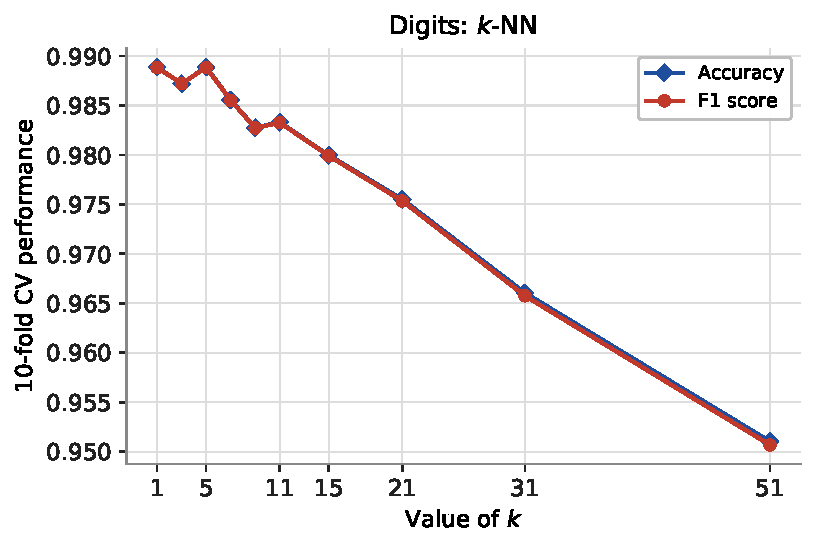
\includegraphics[width=0.6\textwidth]{figures/digits_knn.pdf}
\caption{Digits: $k$-NN accuracy and F1 vs.\ $k$.}
\end{figure}

Best: $k = 5$, accuracy 0.9889, F1 0.9888 ($k = 1$ is the same). Performance falls steadily as $k$ grows,
down to 0.9510 at $k = 51$. Each digit has only about 160 training images, so a large neighborhood starts
including look-alike digits (e.g.\ 3, 8 and 9) and the vote gets worse.

\subsection*{Random forest}
\begin{table}[H]
\centering
\small
\begin{tabular}{lcccccc}
\toprule
\texttt{min\_size}, \texttt{max\_depth} & 2, none & 5, none & 10, none & 20, none & 5, 5 & 5, 10 \\
\midrule
Accuracy & \textbf{0.9493} & 0.9482 & 0.9360 & 0.9310 & 0.8409 & 0.9422 \\
F1 score & \textbf{0.9492} & 0.9480 & 0.9355 & 0.9308 & 0.8369 & 0.9419 \\
\bottomrule
\end{tabular}
\vspace{0.3cm}

\begin{tabular}{lccccccc}
\toprule
$ntree$ & 1 & 5 & 10 & 20 & 30 & 40 & 50 \\
\midrule
Accuracy & 0.7745 & 0.9131 & 0.9504 & 0.9704 & 0.9760 & 0.9738 & \textbf{0.9771} \\
F1 score & 0.7715 & 0.9114 & 0.9495 & 0.9704 & 0.9760 & 0.9737 & \textbf{0.9770} \\
\bottomrule
\end{tabular}
\caption{Digits:random forest. Top: 6 stopping criteria at $ntree = 10$. Bottom: 7 values of $ntree$ with the best stopping criterion. Bold is the best value.}
\end{table}

\begin{figure}[H]
\centering
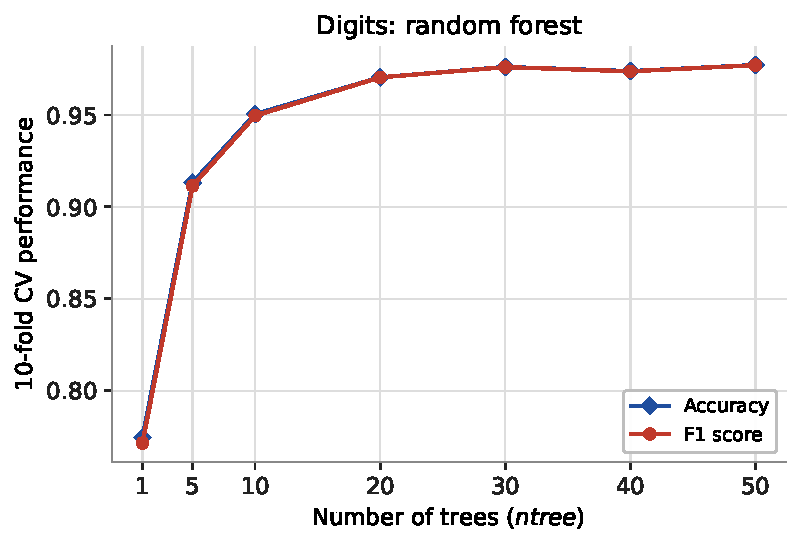
\includegraphics[width=0.6\textwidth]{figures/digits_rf.pdf}
\caption{Digits: random forest accuracy and F1 vs.\ $ntree$ (\texttt{min\_size} = 2, no max depth).}
\end{figure}

Best stopping criterion: \texttt{minimum\_size\_for\_split} = 2 (full trees). \texttt{maximum\_depth} = 5 is
by far the worst (0.8409), because separating 10 classes needs deep trees. Best: $ntree = 50$, accuracy 0.9771,
F1 0.9770. This is the dataset where $ntree$ matters most: one tree gets only 0.7745, since it only sees 8 random
pixels per split and one mean threshold, but averaging 50 of them adds 0.20. The curve is still rising slightly at 50.

\subsection*{Neural network}
\begin{table}[H]
\centering
\small
\begin{tabular}{lcccccc}
\toprule
Network & \multicolumn{2}{c}{$\lambda = 0$} & \multicolumn{2}{c}{$\lambda = 0.1$} & \multicolumn{2}{c}{$\lambda = 1$} \\
\cmidrule(lr){2-3} \cmidrule(lr){4-5} \cmidrule(lr){6-7}
 & Acc. & F1 & Acc. & F1 & Acc. & F1 \\
\midrule
{[64 8 10]} & 0.9560 & 0.9561 & 0.9588 & 0.9588 & 0.9676 & 0.9676 \\
{[64 16 10]} & 0.9732 & 0.9732 & 0.9743 & 0.9743 & 0.9738 & 0.9738 \\
{[64 32 10]} & 0.9793 & 0.9793 & 0.9799 & 0.9798 & 0.9766 & 0.9765 \\
{[64 64 10]} & 0.9816 & 0.9816 & \textbf{0.9821} & \textbf{0.9821} & 0.9760 & 0.9760 \\
{[64 16 16 10]} & 0.9738 & 0.9738 & 0.9755 & 0.9756 & 0.9738 & 0.9738 \\
{[64 32 32 10]} & 0.9788 & 0.9787 & 0.9788 & 0.9787 & 0.9759 & 0.9759 \\
\bottomrule
\end{tabular}
\caption{Digits:neural network, $\alpha = 0.3$, $m = 300$ epochs, mini-batch 32. Bold is the best value.}
\end{table}

\begin{figure}[H]
\centering
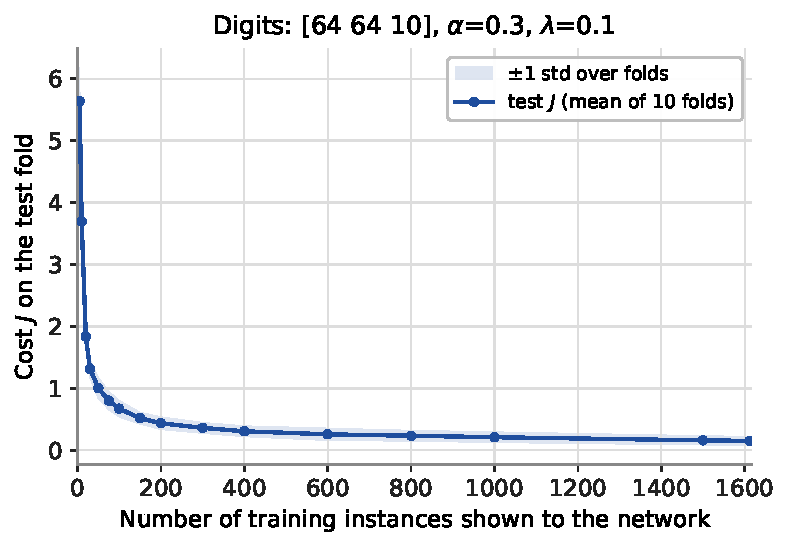
\includegraphics[width=0.6\textwidth]{figures/digits_nn_curve.pdf}
\caption{Digits: learning curve of $[64\ 64\ 10]$, $\lambda = 0.1$, $\alpha = 0.3$. Cost $J$ on the test fold vs.\
number of training instances, mean of 10 folds.}
\end{figure}

$\alpha = 0.3$, $m = 300$ epochs. Best: $[64\ 64\ 10]$ with $\lambda = 0.1$, accuracy 0.9821, F1 0.9821. Width
is what matters: one hidden layer goes 0.9560, 0.9732, 0.9793, 0.9816 for 8, 16, 32, 64 neurons ($\lambda = 0$),
since 8 hidden neurons are too few to separate 10 classes. A second layer does not help (0.9788 for
$[64\ 32\ 32\ 10]$). $\lambda$ changes little except for the smallest network.

Learning curve: $J$ is 5.64 with 5 instances (with 10 outputs, $J$ adds up 10 error terms, and 5 images cannot
cover 10 digits), 1.00 with 50, 0.36 with 300 and 0.15 with all 1612. It is still going down at the end, so more
images would still help.

\textbf{Best for Digits:} $k$-NN ($k = 5$). With pixels on the same scale, the distance already captures what
makes two digits alike, and $k$-NN uses every training image directly.

%-------------------------------------------------------------
\newpage
\section{The Oxford Parkinson's Disease Detection Dataset}

195 voice recordings, 22 numerical attributes, 147 Parkinson's (positive class) and 48 healthy.

\textbf{Algorithms and why.} The dataset is small and fully numerical, so $k$-NN with normalized attributes is
a natural first choice. The random forest handles attributes on very different scales without
normalizing, and the neural network can combine all 22 voice measurements. One thing to note: the 195
recordings come from only 31 people (about 6 each), and the folds split recordings, not people, so the same
person is usually in both the training and test folds.

\subsection*{$k$-NN}
\begin{table}[H]
\centering
\small
\begin{tabular}{lcccccccccc}
\toprule
$k$ & 1 & 3 & 5 & 7 & 9 & 11 & 15 & 21 & 31 & 51 \\
\midrule
Accuracy & \textbf{0.9594} & 0.9283 & 0.9233 & 0.9239 & 0.9244 & 0.9039 & 0.8525 & 0.8101 & 0.8412 & 0.7851 \\
F1 score & \textbf{0.9720} & 0.9523 & 0.9503 & 0.9519 & 0.9516 & 0.9391 & 0.9086 & 0.8862 & 0.9055 & 0.8754 \\
\bottomrule
\end{tabular}
\caption{Parkinsons:$k$-NN, 10-fold stratified CV, for 10 values of $k$. Bold is the best value.}
\end{table}

\begin{figure}[H]
\centering
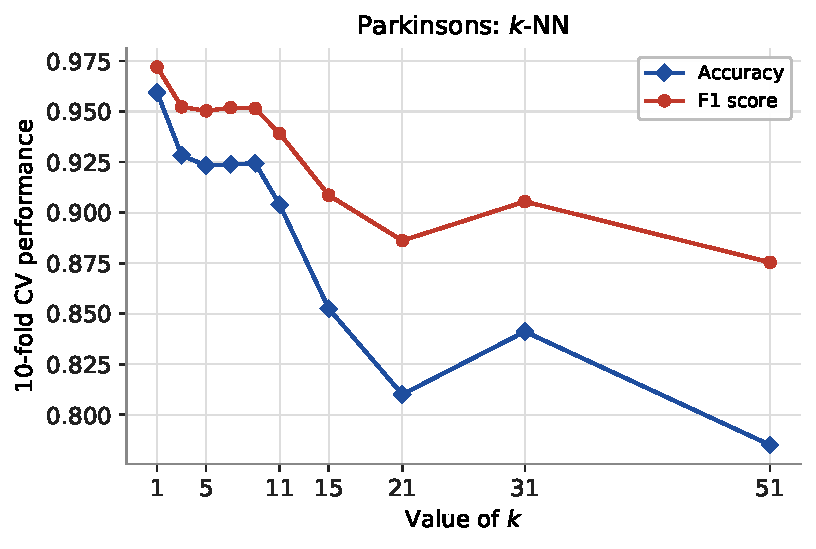
\includegraphics[width=0.6\textwidth]{figures/parkinsons_knn.pdf}
\caption{Parkinsons: $k$-NN accuracy and F1 vs.\ $k$.}
\end{figure}

Best: $k = 1$, accuracy 0.9594, F1 0.9720. This is because of the repeated recordings: the nearest neighbor
of a test recording is usually another recording of the same person, which has the right label. With larger
$k$, accuracy drops to 0.7851 at $k = 51$, faster than F1, because the 48 healthy recordings get outvoted by the
majority class.

\subsection*{Random forest}
\begin{table}[H]
\centering
\small
\begin{tabular}{lcccccc}
\toprule
\texttt{min\_size}, \texttt{max\_depth} & 2, none & 5, none & 10, none & 20, none & 5, 5 & 5, 10 \\
\midrule
Accuracy & 0.8820 & 0.8925 & \textbf{0.8984} & 0.8681 & 0.8825 & 0.8925 \\
F1 score & 0.9241 & 0.9297 & \textbf{0.9346} & 0.9155 & 0.9241 & 0.9297 \\
\bottomrule
\end{tabular}
\vspace{0.3cm}

\begin{tabular}{lccccccc}
\toprule
$ntree$ & 1 & 5 & 10 & 20 & 30 & 40 & 50 \\
\midrule
Accuracy & 0.8447 & 0.8723 & 0.9025 & 0.8975 & \textbf{0.9031} & 0.8981 & 0.8831 \\
F1 score & 0.8977 & 0.9161 & 0.9375 & 0.9356 & \textbf{0.9393} & 0.9343 & 0.9249 \\
\bottomrule
\end{tabular}
\caption{Parkinsons:random forest. Top: 6 stopping criteria at $ntree = 10$. Bottom: 7 values of $ntree$ with the best stopping criterion. Bold is the best value.}
\end{table}

\begin{figure}[H]
\centering
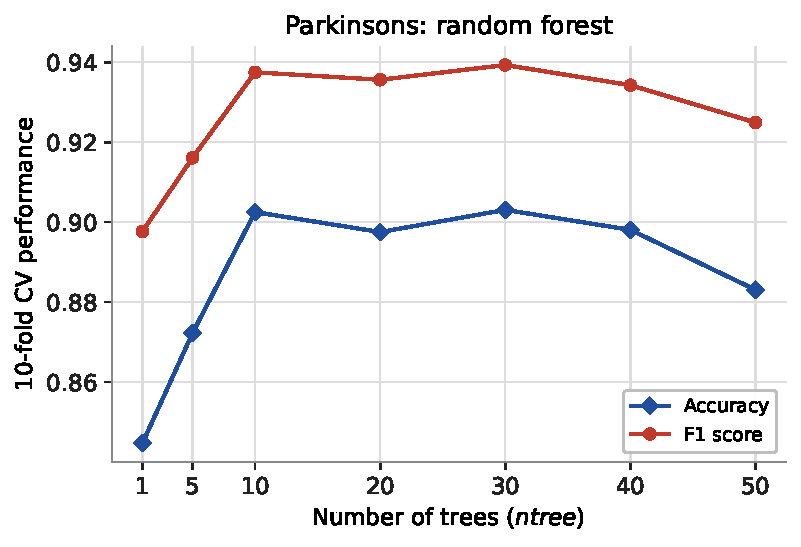
\includegraphics[width=0.6\textwidth]{figures/parkinsons_rf.pdf}
\caption{Parkinsons: random forest accuracy and F1 vs.\ $ntree$ (\texttt{min\_size} = 10).}
\end{figure}

Best stopping criterion: \texttt{minimum\_size\_for\_split} = 10. Best: $ntree = 30$, accuracy 0.9031, F1 0.9393.
Most of the gain is by 10 trees. The drop at 50 trees (0.8831) is noise: each test fold has only about 20
recordings, so one recording is 0.05 accuracy on that fold.

\subsection*{Neural network}
\begin{table}[H]
\centering
\small
\begin{tabular}{lcccccc}
\toprule
Network & \multicolumn{2}{c}{$\lambda = 0$} & \multicolumn{2}{c}{$\lambda = 0.1$} & \multicolumn{2}{c}{$\lambda = 1$} \\
\cmidrule(lr){2-3} \cmidrule(lr){4-5} \cmidrule(lr){6-7}
 & Acc. & F1 & Acc. & F1 & Acc. & F1 \\
\midrule
{[22 8 1]} & 0.8983 & 0.9287 & 0.8517 & 0.8976 & 0.8209 & 0.8779 \\
{[22 16 1]} & 0.9039 & 0.9377 & 0.8678 & 0.9165 & 0.8365 & 0.9013 \\
{[22 32 1]} & 0.9089 & 0.9407 & 0.8511 & 0.9039 & 0.7854 & 0.8619 \\
{[22 64 1]} & 0.9134 & \textbf{0.9442} & 0.8473 & 0.8992 & 0.7515 & 0.8133 \\
{[22 16 16 1]} & 0.9028 & 0.9333 & 0.8526 & 0.9061 & 0.8204 & 0.8883 \\
{[22 32 32 1]} & \textbf{0.9144} & 0.9440 & 0.8331 & 0.8910 & 0.7204 & 0.7729 \\
\bottomrule
\end{tabular}
\caption{Parkinsons:neural network, $\alpha = 3$, $m = 300$ epochs, mini-batch 32. Bold is the best value.}
\end{table}

\begin{figure}[H]
\centering
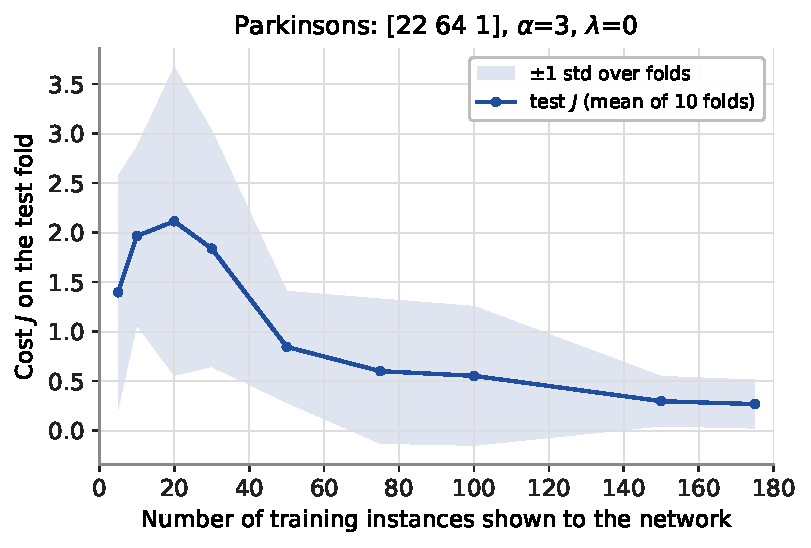
\includegraphics[width=0.6\textwidth]{figures/parkinsons_nn_curve.pdf}
\caption{Parkinsons: learning curve of $[22\ 64\ 1]$, $\lambda = 0$, $\alpha = 3$. Cost $J$ on the test fold vs.\
number of training instances, mean of 10 folds.}
\end{figure}

$\alpha = 3$, $m = 300$ epochs. The large step size is needed because 175 training instances is only 6
mini-batches per epoch, so smaller $\alpha$ does not converge in 300 epochs. Best: $[22\ 64\ 1]$ with $\lambda = 0$,
accuracy 0.9134, F1 0.9442. Regularization hurts every network (e.g.\ $[22\ 64\ 1]$ goes 0.9134, 0.8473, 0.7515
for $\lambda = 0, 0.1, 1$). The penalty is $\frac{\lambda}{2n}$ with a small $n$, so it is strong here, and it
pushes the network toward predicting the majority class.

Learning curve: $J$ first goes up from 1.40 to 2.11 between 5 and 20 instances (the network becomes confidently
wrong after a full training run on a few recordings, like in HW4), then falls to 0.27 with all 175. The std band
is wide because each test fold has only about 20 recordings.

\textbf{Best for Parkinsons:} $k$-NN ($k = 1$). Since the folds put the same person on both sides, this score is
optimistic for a new patient: it rewards recognizing a person more than recognizing the disease.

%-------------------------------------------------------------
\newpage
\section{The Rice Grains Dataset}

3810 grains, 7 numerical attributes, 1630 Cammeo (positive class) and 2180 Osmancik.

\textbf{Algorithms and why.} Few numerical attributes and many instances is a good setting for all three:
$k$-NN has plenty of neighbors, the random forest can split on the 7 shape measurements directly, and the
neural network has enough data to fit a boundary without much overfitting.

\subsection*{$k$-NN}
\begin{table}[H]
\centering
\small
\begin{tabular}{lcccccccccc}
\toprule
$k$ & 1 & 3 & 5 & 7 & 9 & 11 & 15 & 21 & 31 & 51 \\
\midrule
Accuracy & 0.8858 & 0.9129 & 0.9189 & 0.9215 & 0.9236 & 0.9247 & 0.9273 & 0.9273 & 0.9278 & \textbf{0.9286} \\
F1 score & 0.8673 & 0.8979 & 0.9049 & 0.9080 & 0.9104 & 0.9116 & 0.9145 & 0.9145 & 0.9153 & \textbf{0.9163} \\
\bottomrule
\end{tabular}
\caption{Rice:$k$-NN, 10-fold stratified CV, for 10 values of $k$. Bold is the best value.}
\end{table}

\begin{figure}[H]
\centering
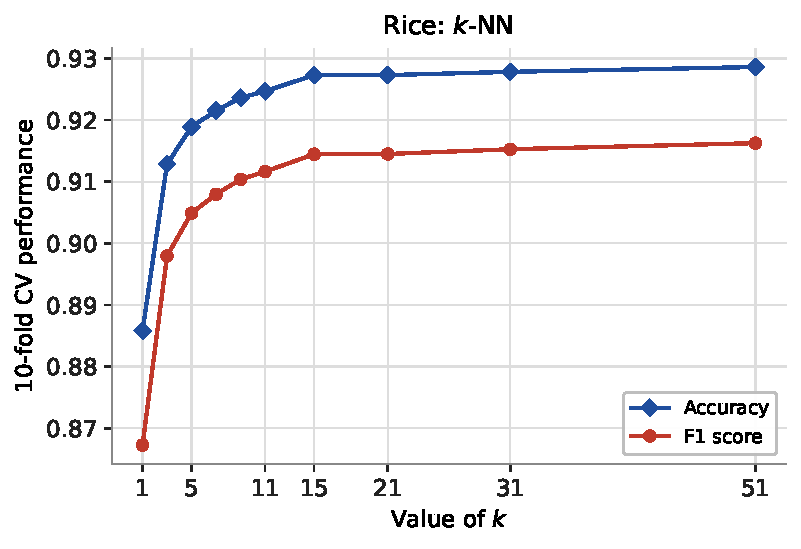
\includegraphics[width=0.6\textwidth]{figures/rice_knn.pdf}
\caption{Rice: $k$-NN accuracy and F1 vs.\ $k$.}
\end{figure}

Best: $k = 51$, accuracy 0.9286, F1 0.9163. Unlike Digits, performance goes up with $k$: 0.8858 at $k = 1$. The
two species overlap in shape, so the single nearest grain is often of the other species, and a larger vote
averages that out. The curve is flat from $k = 15$ (0.9273 to 0.9286), so a larger $k$ would not change much.

\subsection*{Random forest}
\begin{table}[H]
\centering
\small
\begin{tabular}{lcccccc}
\toprule
\texttt{min\_size}, \texttt{max\_depth} & 2, none & 5, none & 10, none & 20, none & 5, 5 & 5, 10 \\
\midrule
Accuracy & 0.9144 & 0.9197 & 0.9215 & \textbf{0.9255} & 0.9241 & 0.9147 \\
F1 score & 0.8995 & 0.9059 & 0.9074 & \textbf{0.9124} & 0.9106 & 0.8998 \\
\bottomrule
\end{tabular}
\vspace{0.3cm}

\begin{tabular}{lccccccc}
\toprule
$ntree$ & 1 & 5 & 10 & 20 & 30 & 40 & 50 \\
\midrule
Accuracy & 0.9184 & 0.9252 & 0.9268 & 0.9273 & \textbf{0.9302} & 0.9278 & 0.9276 \\
F1 score & 0.9041 & 0.9120 & 0.9141 & 0.9149 & \textbf{0.9182} & 0.9154 & 0.9151 \\
\bottomrule
\end{tabular}
\caption{Rice:random forest. Top: 6 stopping criteria at $ntree = 10$. Bottom: 7 values of $ntree$ with the best stopping criterion. Bold is the best value.}
\end{table}

\begin{figure}[H]
\centering
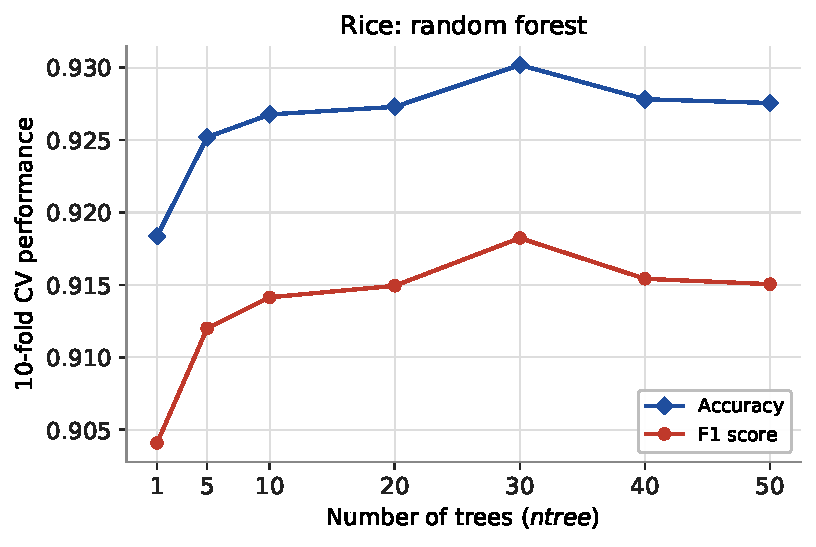
\includegraphics[width=0.6\textwidth]{figures/rice_rf.pdf}
\caption{Rice: random forest accuracy and F1 vs.\ $ntree$ (\texttt{min\_size} = 20).}
\end{figure}

Best stopping criterion: \texttt{minimum\_size\_for\_split} = 20, the largest one tested; bigger leaves stop the trees from
fitting the overlap between species. Best: $ntree = 30$, accuracy 0.9302, F1 0.9182. Even one tree gets 0.9184,
with 3429 training grains and only 7 attributes, so voting adds only 0.012.

\subsection*{Neural network}
\begin{table}[H]
\centering
\small
\begin{tabular}{lcccccc}
\toprule
Network & \multicolumn{2}{c}{$\lambda = 0$} & \multicolumn{2}{c}{$\lambda = 0.1$} & \multicolumn{2}{c}{$\lambda = 1$} \\
\cmidrule(lr){2-3} \cmidrule(lr){4-5} \cmidrule(lr){6-7}
 & Acc. & F1 & Acc. & F1 & Acc. & F1 \\
\midrule
{[7 8 1]} & 0.9252 & 0.9124 & 0.9252 & 0.9124 & 0.9255 & 0.9126 \\
{[7 16 1]} & \textbf{0.9260} & 0.9130 & 0.9257 & 0.9127 & 0.9249 & 0.9116 \\
{[7 32 1]} & 0.9257 & 0.9132 & \textbf{0.9260} & \textbf{0.9133} & 0.9241 & 0.9109 \\
{[7 64 1]} & 0.9228 & 0.9093 & 0.9223 & 0.9086 & 0.9197 & 0.9055 \\
{[7 16 16 1]} & 0.9255 & 0.9130 & 0.9234 & 0.9105 & 0.9186 & 0.9054 \\
{[7 32 32 1]} & 0.9189 & 0.9030 & 0.9181 & 0.9020 & 0.9115 & 0.8936 \\
\bottomrule
\end{tabular}
\caption{Rice:neural network, $\alpha = 0.3$, $m = 300$ epochs, mini-batch 32. Bold is the best value.}
\end{table}

\begin{figure}[H]
\centering
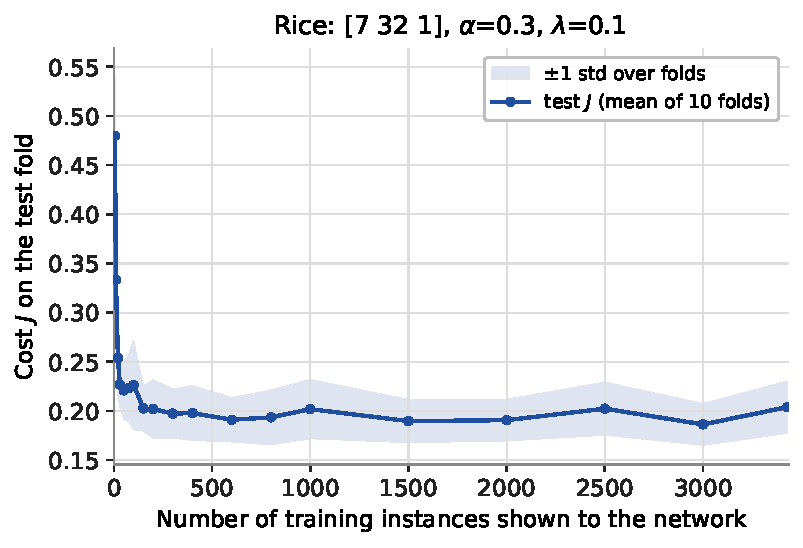
\includegraphics[width=0.6\textwidth]{figures/rice_nn_curve.pdf}
\caption{Rice: learning curve of $[7\ 32\ 1]$, $\lambda = 0.1$, $\alpha = 0.3$. Cost $J$ on the test fold vs.\
number of training instances, mean of 10 folds.}
\end{figure}

$\alpha = 0.3$, $m = 300$ epochs. Best: $[7\ 32\ 1]$ with $\lambda = 0.1$, accuracy 0.9260, F1 0.9133. Most networks
are between 0.918 and 0.926, and the biggest, $[7\ 32\ 32\ 1]$, is slightly worse (0.9189). With 7 inputs the
boundary is simple, so a larger network has nothing more to learn.

Learning curve: $J$ falls from 0.48 with 5 instances to 0.22 with 30, then stays at about 0.19 to 0.20 from 150 to all
3429. The network learns the boundary from about 150 grains; the remaining error is the overlap between the two
species, which more data cannot remove.

\textbf{Best for Rice:} random forest ($ntree = 30$), but all three are within 0.005 accuracy. They all reach
the same ceiling of about 0.93, set by the overlap between species, not by the algorithm.

%-------------------------------------------------------------
\newpage
\section{The Credit Approval Dataset}

653 applications, 296 approved (positive class) and 357 rejected. In the csv, 10 attributes are categorical
and 5 numerical (the handout says 9 and 6; we followed the column names). After one-hot encoding there are 68
inputs, since one categorical attribute has 23 values and another 14.

\textbf{Algorithms and why.} This is the only mixed dataset. The random forest is the natural choice since it
splits on categorical attributes directly. The neural network can use the one-hot inputs and learn which ones
matter. $k$-NN is the riskiest, because after one-hot encoding the distance is dominated by the 63 categorical
columns.

\subsection*{$k$-NN}
\begin{table}[H]
\centering
\small
\begin{tabular}{lcccccccccc}
\toprule
$k$ & 1 & 3 & 5 & 7 & 9 & 11 & 15 & 21 & 31 & 51 \\
\midrule
Accuracy & 0.8114 & 0.8512 & \textbf{0.8665} & 0.8649 & 0.8527 & 0.8512 & 0.8528 & 0.8543 & 0.8544 & 0.8559 \\
F1 score & 0.7827 & 0.8326 & \textbf{0.8510} & 0.8496 & 0.8352 & 0.8317 & 0.8328 & 0.8339 & 0.8315 & 0.8291 \\
\bottomrule
\end{tabular}
\caption{Credit:$k$-NN, 10-fold stratified CV, for 10 values of $k$. Bold is the best value.}
\end{table}

\begin{figure}[H]
\centering
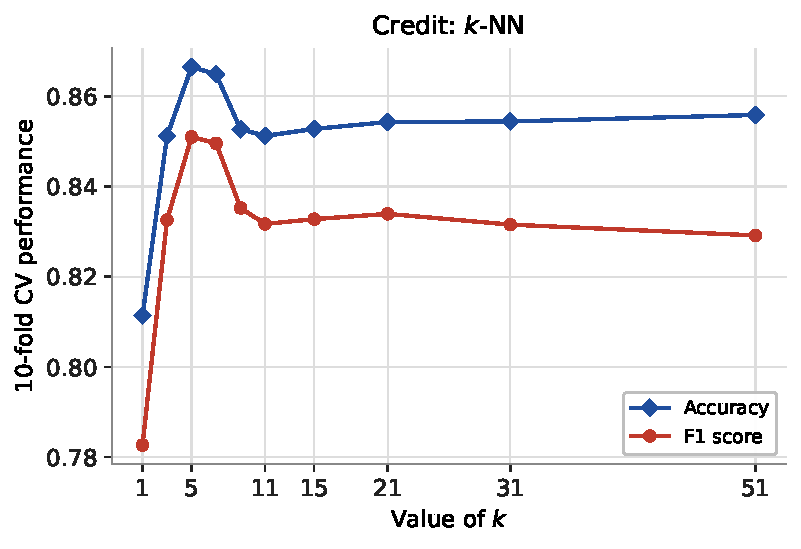
\includegraphics[width=0.6\textwidth]{figures/credit_knn.pdf}
\caption{Credit: $k$-NN accuracy and F1 vs.\ $k$.}
\end{figure}

Best: $k = 5$, accuracy 0.8665, F1 0.8510. $k = 1$ is clearly worse (0.8114), and after $k = 7$ the curve is flat at about
0.85. Each categorical mismatch adds 1 to two one-hot columns, while a normalized numerical difference is usually much
smaller than 1. So neighbors are mostly chosen by matching categories, and the numerical attributes count for little.

\subsection*{Random forest}
\begin{table}[H]
\centering
\small
\begin{tabular}{lcccccc}
\toprule
\texttt{min\_size}, \texttt{max\_depth} & 2, none & 5, none & 10, none & 20, none & 5, 5 & 5, 10 \\
\midrule
Accuracy & 0.8436 & 0.8449 & 0.8482 & 0.8541 & \textbf{0.8544} & 0.8402 \\
F1 score & 0.8234 & 0.8297 & 0.8274 & 0.8355 & \textbf{0.8382} & 0.8231 \\
\bottomrule
\end{tabular}
\vspace{0.3cm}

\begin{tabular}{lccccccc}
\toprule
$ntree$ & 1 & 5 & 10 & 20 & 30 & 40 & 50 \\
\midrule
Accuracy & 0.7853 & 0.8405 & 0.8391 & 0.8635 & \textbf{0.8697} & 0.8604 & 0.8635 \\
F1 score & 0.7548 & 0.8174 & 0.8162 & 0.8454 & \textbf{0.8542} & 0.8448 & 0.8484 \\
\bottomrule
\end{tabular}
\caption{Credit:random forest. Top: 6 stopping criteria at $ntree = 10$. Bottom: 7 values of $ntree$ with the best stopping criterion. Bold is the best value.}
\end{table}

\begin{figure}[H]
\centering
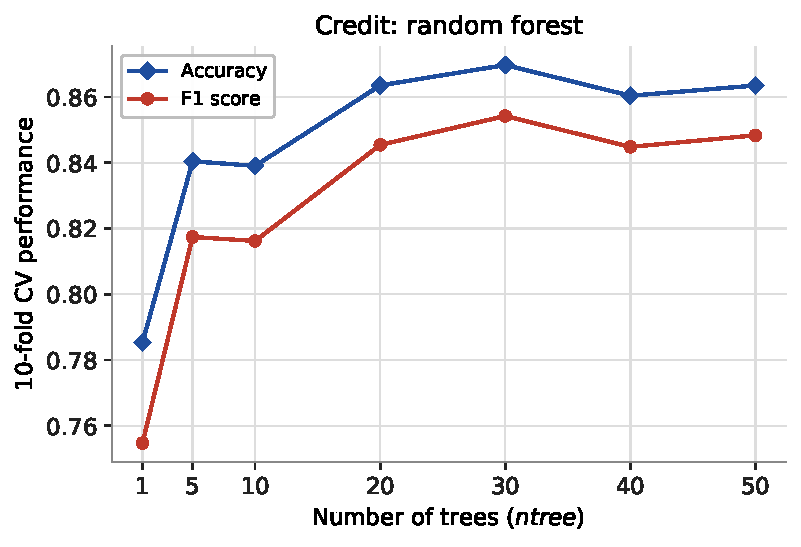
\includegraphics[width=0.6\textwidth]{figures/credit_rf.pdf}
\caption{Credit: random forest accuracy and F1 vs.\ $ntree$ (\texttt{min\_size} = 5, \texttt{max\_depth} = 5).}
\end{figure}

Best stopping criterion: \texttt{maximum\_depth} = 5. Shallow trees work best because a categorical split with
23 values creates many small children that are easy to overfit. Best: $ntree = 30$, accuracy 0.8697, F1 0.8542.
Accuracy goes from 0.7853 with one tree to 0.8697, then stays within 0.01.

\subsection*{Neural network}
\begin{table}[H]
\centering
\small
\begin{tabular}{lcccccc}
\toprule
Network & \multicolumn{2}{c}{$\lambda = 0$} & \multicolumn{2}{c}{$\lambda = 0.1$} & \multicolumn{2}{c}{$\lambda = 1$} \\
\cmidrule(lr){2-3} \cmidrule(lr){4-5} \cmidrule(lr){6-7}
 & Acc. & F1 & Acc. & F1 & Acc. & F1 \\
\midrule
{[68 8 1]} & 0.8496 & 0.8363 & 0.8542 & 0.8425 & 0.8558 & 0.8461 \\
{[68 16 1]} & 0.8605 & 0.8480 & 0.8605 & 0.8480 & 0.8604 & 0.8516 \\
{[68 32 1]} & 0.8619 & 0.8467 & 0.8681 & 0.8547 & \textbf{0.8728} & \textbf{0.8631} \\
{[68 64 1]} & 0.8572 & 0.8450 & 0.8556 & 0.8434 & 0.8650 & 0.8579 \\
{[68 16 16 1]} & 0.8590 & 0.8399 & 0.8559 & 0.8367 & 0.8482 & 0.8313 \\
{[68 32 32 1]} & 0.8528 & 0.8410 & 0.8590 & 0.8483 & 0.8558 & 0.8499 \\
\bottomrule
\end{tabular}
\caption{Credit:neural network, $\alpha = 0.3$, $m = 100$ epochs, mini-batch 32. Bold is the best value.}
\end{table}

\begin{figure}[H]
\centering
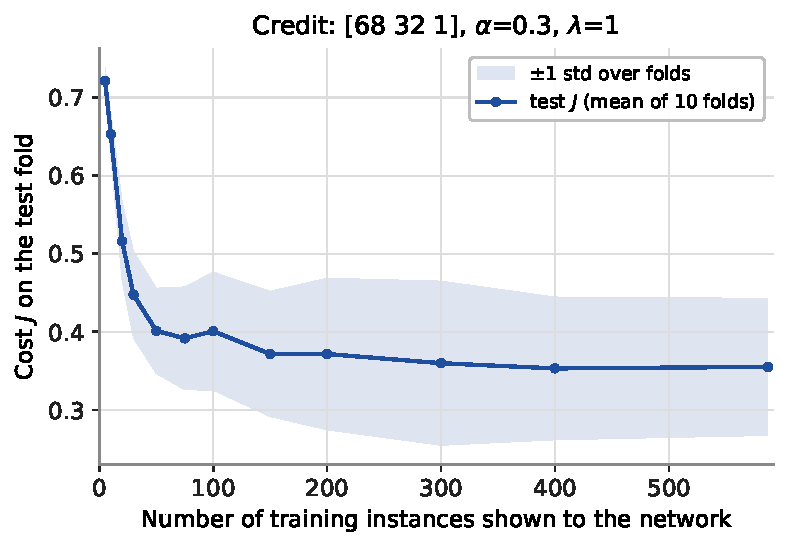
\includegraphics[width=0.6\textwidth]{figures/credit_nn_curve.pdf}
\caption{Credit: learning curve of $[68\ 32\ 1]$, $\lambda = 1$, $\alpha = 0.3$. Cost $J$ on the test fold vs.\
number of training instances, mean of 10 folds.}
\end{figure}

$\alpha = 0.3$, $m = 100$ epochs (300 epochs overfits: 0.8422). Best: $[68\ 32\ 1]$ with $\lambda = 1$, accuracy
0.8728, F1 0.8631. This is the only dataset where the largest $\lambda$ wins. Many one-hot inputs are rare categories
that only a few applicants have, which the network can memorize, and regularization keeps those weights small.

Learning curve: $J$ falls from 0.72 with 5 instances to 0.40 with 50, then slowly to 0.355 with all 587, with little
change after about 300 instances.

\textbf{Best for Credit:} neural network ($[68\ 32\ 1]$, $\lambda = 1$), with the random forest close behind.
Both handle the mixed attributes better than $k$-NN, whose distance does not suit one-hot inputs.

%-------------------------------------------------------------
\newpage
\section{Summary}

\begin{table}[H]
\centering
\small
\begin{tabular}{l cc cc cc cc}
\toprule
 & \multicolumn{2}{c}{Digits} & \multicolumn{2}{c}{Parkinsons} & \multicolumn{2}{c}{Rice} & \multicolumn{2}{c}{Credit} \\
\cmidrule(lr){2-3} \cmidrule(lr){4-5} \cmidrule(lr){6-7} \cmidrule(lr){8-9}
 & Accuracy & F1 score & Accuracy & F1 score & Accuracy & F1 score & Accuracy & F1 score \\
\midrule
$k$-NN & \cellcolor{gray!30}0.9889 & \cellcolor{gray!30}0.9888 & \cellcolor{gray!30}0.9594 & \cellcolor{gray!30}0.9720 & 0.9286 & 0.9163 & 0.8665 & 0.8510 \\
Random Forest & 0.9771 & 0.9770 & 0.9031 & 0.9393 & \cellcolor{gray!30}0.9302 & \cellcolor{gray!30}0.9182 & 0.8697 & 0.8542 \\
Neural Network & 0.9821 & 0.9821 & 0.9134 & 0.9442 & 0.9260 & 0.9133 & \cellcolor{gray!30}0.8728 & \cellcolor{gray!30}0.8631 \\
\midrule
\textcolor{red}{Ensemble (EC 3)} & 0.9827 & 0.9827 & 0.9128 & 0.9430 & 0.9289 & 0.9167 & 0.8574 & 0.8476 \\
\bottomrule
\end{tabular}
\caption{Best setting of each algorithm, 10-fold stratified CV. Gray is the best algorithm for that dataset and metric (among $k$-NN, random forest and neural network).}
\end{table}

There is no single best algorithm. $k$-NN wins on the two datasets where the distance is meaningful: Digits, with
all pixels on the same scale, and Parkinsons, where it can match recordings of the same person. On Rice all three
algorithms reach the same ceiling of about 0.93, and the random forest is only slightly ahead. On Credit, the only
mixed dataset, the neural network and the random forest beat $k$-NN, whose distance does not suit one-hot inputs.

%-------------------------------------------------------------
\section*{\textcolor{red}{Extra Credit}}

\subsection*{\textcolor{red}{Extra Credit 1: a third algorithm on every dataset}}

We evaluated three algorithms on all four datasets ($k$-NN, random forest, neural network), each with at least 6
hyperparameter settings and its own graph (Sections 1 to 4).

\subsection*{\textcolor{red}{Extra Credit 2: a new challenging dataset (Contraceptive Method Choice)}}

\textbf{Dataset.} The UCI Contraceptive Method Choice dataset (a subset of the 1987 National Indonesia
Contraceptive Prevalence Survey). It has 1473 married women, 2 numerical attributes (age, number of children) and
7 categorical ones (wife's and husband's education, religion, working or not, husband's occupation,
standard-of-living index, media exposure). The task is to predict which method she uses, out of 3 classes:
no use (629), long-term (333), short-term (511). So it has both kinds of attributes and more than two classes.
Always predicting ``no use'' gives accuracy 0.427. F1 is macro-F1 over the 3 classes. After one-hot encoding there
are 24 inputs.

\textbf{Algorithms and why.} Same three as the main datasets, with the same tuning. The random forest splits the
categorical attributes directly, the neural network has 3 outputs (one per method), and $k$-NN is the baseline
that should struggle with one-hot inputs, as it did on Credit.

\begin{table}[H]
\centering
\small
\begin{tabular}{lcccccccccc}
\toprule
$k$ & 1 & 3 & 5 & 7 & 9 & 11 & 15 & 21 & 31 & 51 \\
\midrule
Accuracy & 0.4371 & 0.4664 & 0.4672 & 0.4712 & 0.4597 & 0.4665 & 0.4644 & 0.4719 & \textbf{0.4910} & 0.4801 \\
F1 score & 0.4224 & 0.4414 & 0.4486 & 0.4555 & 0.4442 & 0.4490 & 0.4447 & 0.4538 & \textbf{0.4702} & 0.4613 \\
\bottomrule
\end{tabular}
\caption{CMC:$k$-NN, 10-fold stratified CV, for 10 values of $k$. Bold is the best value.}
\end{table}

\begin{figure}[H]
\centering
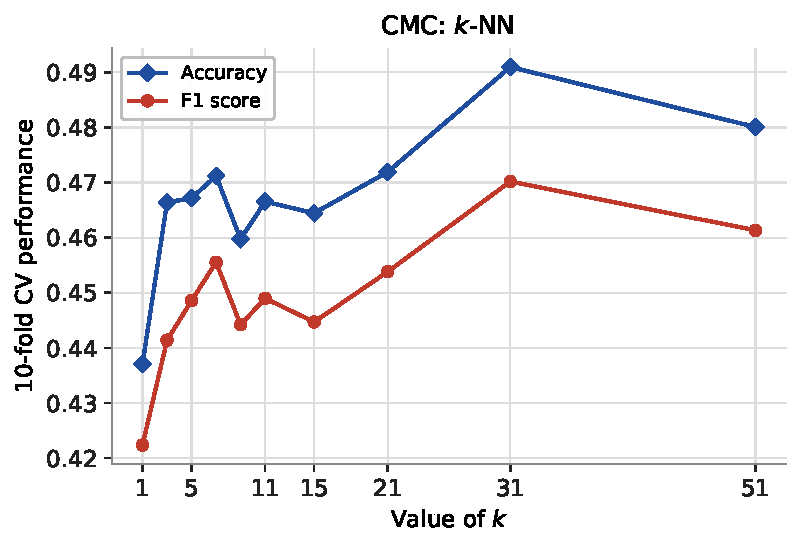
\includegraphics[width=0.6\textwidth]{figures/cmc_knn.pdf}
\caption{CMC: $k$-NN accuracy and F1 vs.\ $k$.}
\end{figure}

$k$-NN, best: $k = 31$, accuracy 0.4910, F1 0.4702. $k = 1$ is only 0.4371, about the majority-class baseline. The
classes overlap so much that a big neighborhood is needed to average out the noise, and the curve is still jumpy.

\begin{table}[H]
\centering
\small
\begin{tabular}{lcccccc}
\toprule
\texttt{min\_size}, \texttt{max\_depth} & 2, none & 5, none & 10, none & 20, none & 5, 5 & 5, 10 \\
\midrule
Accuracy & 0.4793 & 0.5038 & 0.4875 & \textbf{0.5100} & 0.5079 & 0.4773 \\
F1 score & 0.4553 & 0.4810 & 0.4587 & \textbf{0.4870} & 0.4862 & 0.4574 \\
\bottomrule
\end{tabular}
\vspace{0.3cm}

\begin{tabular}{lccccccc}
\toprule
$ntree$ & 1 & 5 & 10 & 20 & 30 & 40 & 50 \\
\midrule
Accuracy & 0.4482 & 0.4902 & 0.5087 & 0.5033 & 0.5107 & 0.5100 & \textbf{0.5114} \\
F1 score & 0.4228 & 0.4645 & 0.4789 & 0.4737 & 0.4869 & 0.4859 & \textbf{0.4891} \\
\bottomrule
\end{tabular}
\caption{CMC:random forest. Top: 6 stopping criteria at $ntree = 10$. Bottom: 7 values of $ntree$ with the best stopping criterion. Bold is the best value.}
\end{table}

\begin{figure}[H]
\centering
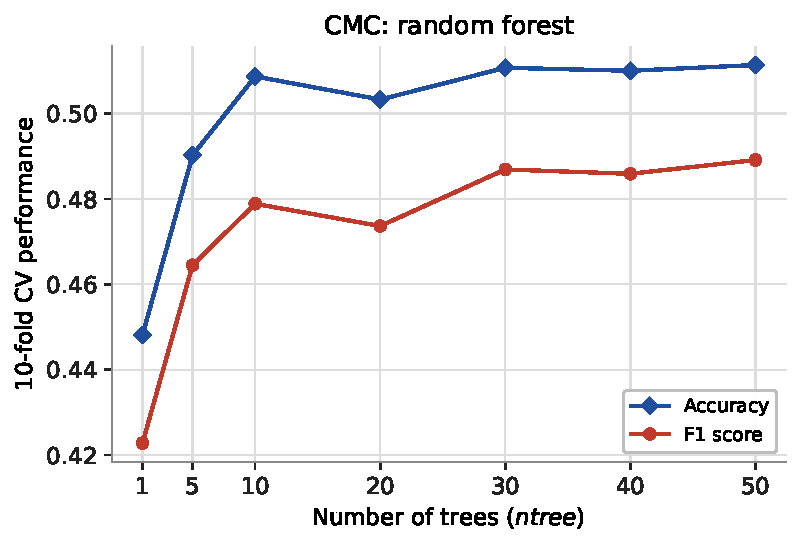
\includegraphics[width=0.6\textwidth]{figures/cmc_rf.pdf}
\caption{CMC: random forest accuracy and F1 vs.\ $ntree$ (\texttt{min\_size} = 20).}
\end{figure}

Random forest, best stopping criterion \texttt{minimum\_size\_for\_split} = 20, best $ntree = 50$: accuracy 0.5114,
F1 0.4891. Large leaves are needed here for the same reason as large $k$ above, and the curve is still rising at 50 trees.

\begin{table}[H]
\centering
\small
\begin{tabular}{lcccccc}
\toprule
Network & \multicolumn{2}{c}{$\lambda = 0$} & \multicolumn{2}{c}{$\lambda = 0.1$} & \multicolumn{2}{c}{$\lambda = 1$} \\
\cmidrule(lr){2-3} \cmidrule(lr){4-5} \cmidrule(lr){6-7}
 & Acc. & F1 & Acc. & F1 & Acc. & F1 \\
\midrule
{[24 8 3]} & 0.5221 & 0.4931 & 0.5290 & 0.4987 & 0.5345 & 0.5035 \\
{[24 16 3]} & 0.5330 & 0.5068 & 0.5330 & 0.5068 & \textbf{0.5439} & \textbf{0.5168} \\
{[24 32 3]} & 0.5134 & 0.4798 & 0.5276 & 0.4952 & 0.5419 & 0.5053 \\
{[24 64 3]} & 0.5201 & 0.4731 & 0.5174 & 0.4644 & 0.5391 & 0.4830 \\
{[24 16 16 3]} & 0.5113 & 0.4899 & 0.5120 & 0.4880 & 0.5100 & 0.4705 \\
{[24 32 32 3]} & 0.5146 & 0.4843 & 0.5201 & 0.4895 & 0.4977 & 0.4220 \\
\bottomrule
\end{tabular}
\caption{CMC:neural network, $\alpha = 0.3$, $m = 300$ epochs, mini-batch 32. Bold is the best value.}
\end{table}

\begin{figure}[H]
\centering
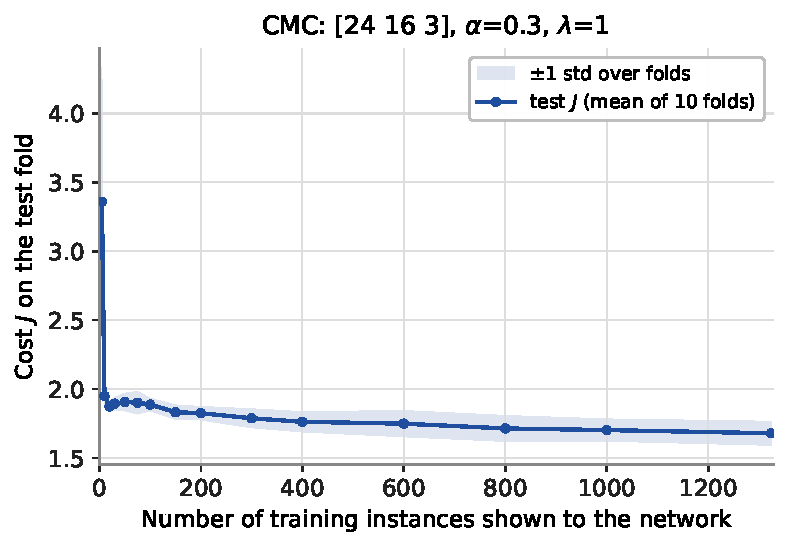
\includegraphics[width=0.6\textwidth]{figures/cmc_nn_curve.pdf}
\caption{CMC: learning curve of $[24\ 16\ 3]$, $\lambda = 1$, $\alpha = 0.3$. Cost $J$ on the test fold vs.\ number of
training instances, mean of 10 folds.}
\end{figure}

Neural network, $\alpha = 0.3$, $m = 300$ epochs. Best: $[24\ 16\ 3]$ with $\lambda = 1$, accuracy 0.5439, F1 0.5168,
the best of the three algorithms. As on Credit, the largest $\lambda$ is best for every one-hidden-layer network, since
the one-hot inputs are easy to memorize; the two-hidden-layer networks are all worse. The learning curve drops from
3.36 to about 1.9 after 10 instances, stays flat until about 100, then falls slowly to 1.68 with all 1324 and is
still going down. The network only finds a weak pattern, and it needs many instances to find even that one.

\textbf{Best for CMC:} neural network, but every algorithm is only about 0.07 to 0.12 above the baseline. The attributes
say little about which method a woman chooses, which is why we picked this as a challenging dataset.

\subsection*{\textcolor{red}{Extra Credit 3: ensemble of different algorithms}}

For each dataset, the ensemble has 5 members: the best $k$-NN, the best random forest, and the 3 best neural
networks with different architectures (all with the hyperparameters found above). In each CV iteration, every member
is trained on its own bootstrap sample of the training folds (drawn with replacement, same size), and the final
prediction is the majority vote of the 5 members.

\begin{table}[H]
\centering
\small
\begin{tabular}{llcc}
\toprule
Dataset & Model (trained on its own bootstrap) & Accuracy & F1 score \\
\midrule
Digits & knn $k$=5 & 0.9811 & 0.9810 \\
 & rf $ntree$=50 & 0.9688 & 0.9686 \\
 & nn 64 $\lambda$=0.1 & 0.9799 & 0.9799 \\
 & nn 32 $\lambda$=0.1 & 0.9749 & 0.9750 \\
 & nn 32-32 $\lambda$=0.1 & 0.9749 & 0.9749 \\
 & \textbf{majority vote of all 5} & 0.9827 & 0.9827 \\
\midrule
Parkinsons & knn $k$=1 & 0.9075 & 0.9389 \\
 & rf $ntree$=30 & 0.8920 & 0.9306 \\
 & nn 64 $\lambda$=0 & 0.8822 & 0.9215 \\
 & nn 32-32 $\lambda$=0 & 0.8975 & 0.9275 \\
 & nn 32 $\lambda$=0 & 0.9033 & 0.9364 \\
 & \textbf{majority vote of all 5} & 0.9128 & 0.9430 \\
\midrule
Rice & knn $k$=51 & 0.9257 & 0.9126 \\
 & rf $ntree$=30 & 0.9257 & 0.9132 \\
 & nn 32 $\lambda$=0.1 & 0.9223 & 0.9105 \\
 & nn 16 $\lambda$=0 & 0.9255 & 0.9122 \\
 & nn 16-16 $\lambda$=0 & 0.9244 & 0.9106 \\
 & \textbf{majority vote of all 5} & 0.9289 & 0.9167 \\
\midrule
Credit & knn $k$=5 & 0.8192 & 0.7946 \\
 & rf $ntree$=30 & 0.8480 & 0.8337 \\
 & nn 32 $\lambda$=1 & 0.8451 & 0.8319 \\
 & nn 64 $\lambda$=1 & 0.8604 & 0.8526 \\
 & nn 16 $\lambda$=1 & 0.8437 & 0.8333 \\
 & \textbf{majority vote of all 5} & 0.8574 & 0.8476 \\

\bottomrule
\end{tabular}
\caption{Extra credit 3: ensemble of $k$-NN, random forest and 3 neural networks (nets named by hidden layers), 10-fold stratified CV.}
\end{table}

The vote is better than every one of its members on Digits, Parkinsons and Rice, and on Credit it is
behind only the $[68\ 64\ 1]$ network. But it never beats the best single algorithm trained on all the training data
(summary table). Bootstrapping costs each member about 37\% of the distinct training instances, and that hurts
$k$-NN the most: on Parkinsons, $k = 1$ drops from 0.9594 to 0.9075 because the matching recording of the same
person is often left out. The vote mostly gets back what the bootstrap took away. On the extra dataset (CMC) the
ensemble gets 0.5261 / 0.4943, again better than each of its members.

\subsection*{\textcolor{red}{Extra Credit 4: a new variant, Extremely Randomized Trees}}

\textbf{What we implemented.} Extra trees (Geurts et al., 2006), a variant of the HW3 random forest, in
extra\_trees.py. Two changes:
\begin{itemize}
\item \textbf{No bootstrap.} Every tree is trained on the whole training set.
\item \textbf{Random thresholds.} For each of the $m$ candidate numerical attributes at a node, the threshold is drawn
uniformly between that attribute's min and max in the node, instead of the mean. The best of the $m$ random cuts by
Information Gain is used. Categorical attributes are split the same way as in HW3.
\end{itemize}
The trees are more random but each one sees all the data, so the variance comes from the random cuts instead of
from the bootstrap. Prediction is the same majority vote. We tuned it exactly like the random forest (6 stopping
criteria at $ntree = 10$, then 7 values of $ntree$) on all five datasets.

\begin{table}[H]
\centering
\small
\begin{tabular}{l cccc cccc}
\toprule
 & \multicolumn{4}{c}{Random forest (HW3)} & \multicolumn{4}{c}{Extra trees} \\
\cmidrule(lr){2-5} \cmidrule(lr){6-9}
Dataset & $ntree$ & Accuracy & F1 score & sec. & $ntree$ & Accuracy & F1 score & sec. \\
\midrule
Digits & 50 & 0.9771 & 0.9770 & 12.9 & 50 & \textbf{0.9832} & \textbf{0.9832} & 17.0 \\
Parkinsons & 30 & 0.9031 & 0.9393 & 0.5 & 30 & \textbf{0.9383} & \textbf{0.9609} & 1.1 \\
Rice & 30 & \textbf{0.9302} & \textbf{0.9182} & 1.6 & 40 & 0.9283 & 0.9160 & 1.7 \\
Credit & 30 & \textbf{0.8697} & \textbf{0.8542} & 1.1 & 30 & 0.8605 & 0.8495 & 1.3 \\
CMC & 50 & \textbf{0.5114} & \textbf{0.4891} & 1.6 & 50 & 0.4957 & 0.4778 & 1.5 \\
\bottomrule
\end{tabular}
\caption{Extra credit 4: best setting of the random forest and of extra trees (each with its own best stopping criterion), 10-fold stratified CV. sec.\ = mean seconds to train 50 trees on one training split. Bold is the better of the two.}
\end{table}

\begin{figure}[H]
\centering
\begin{subfigure}{0.48\textwidth}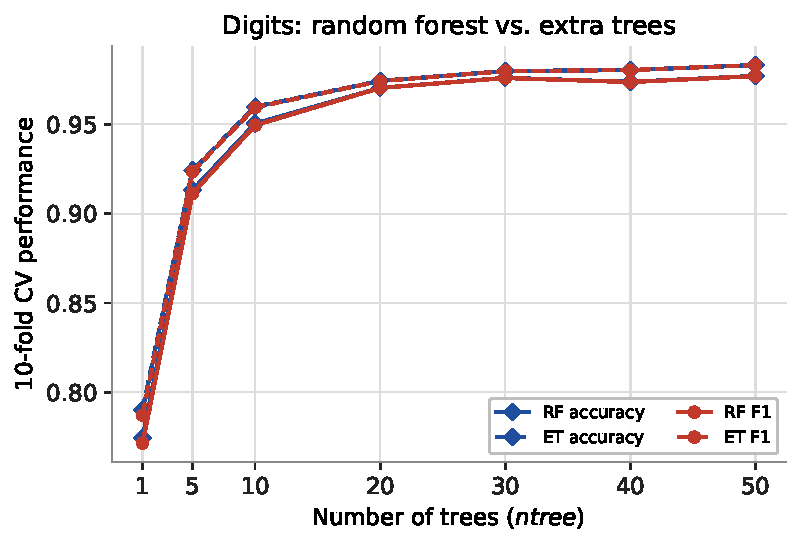
\includegraphics[width=\textwidth]{figures/digits_et.pdf}\end{subfigure}
\begin{subfigure}{0.48\textwidth}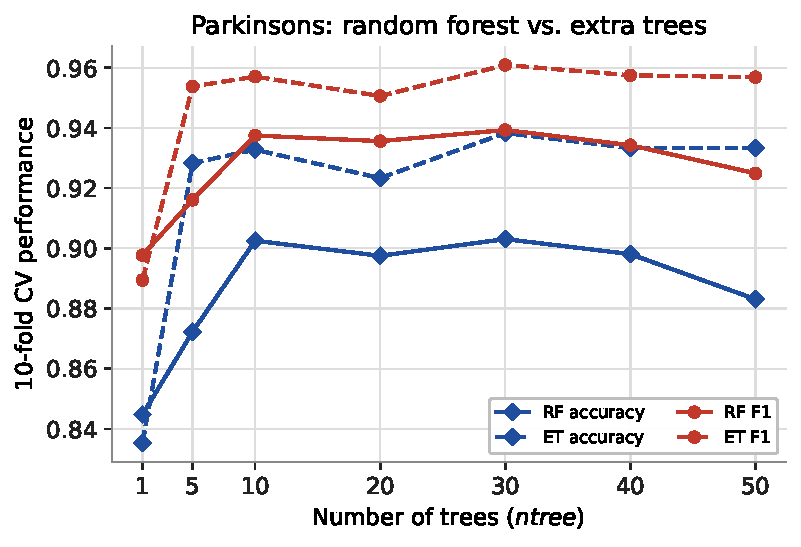
\includegraphics[width=\textwidth]{figures/parkinsons_et.pdf}\end{subfigure}
\begin{subfigure}{0.48\textwidth}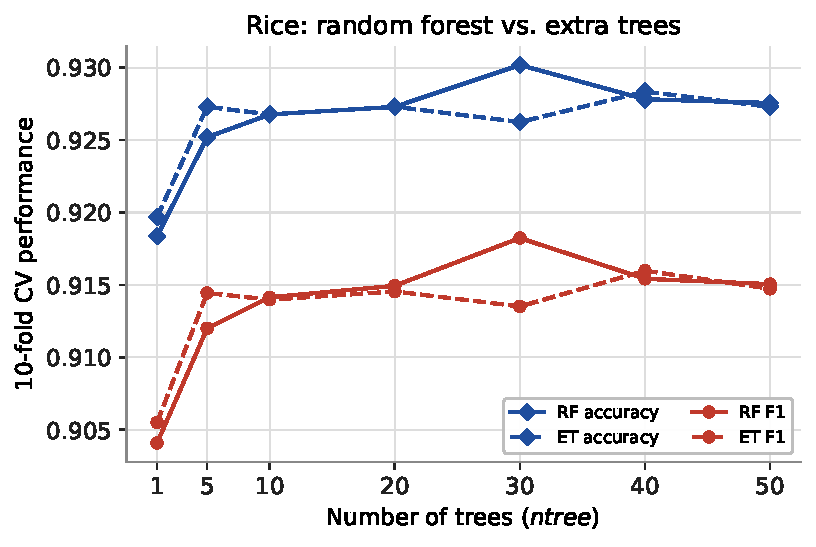
\includegraphics[width=\textwidth]{figures/rice_et.pdf}\end{subfigure}
\begin{subfigure}{0.48\textwidth}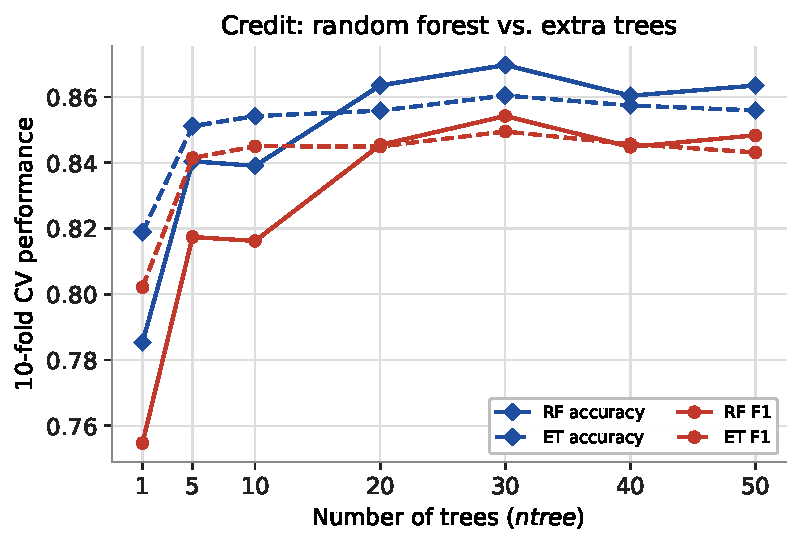
\includegraphics[width=\textwidth]{figures/credit_et.pdf}\end{subfigure}
\begin{subfigure}{0.48\textwidth}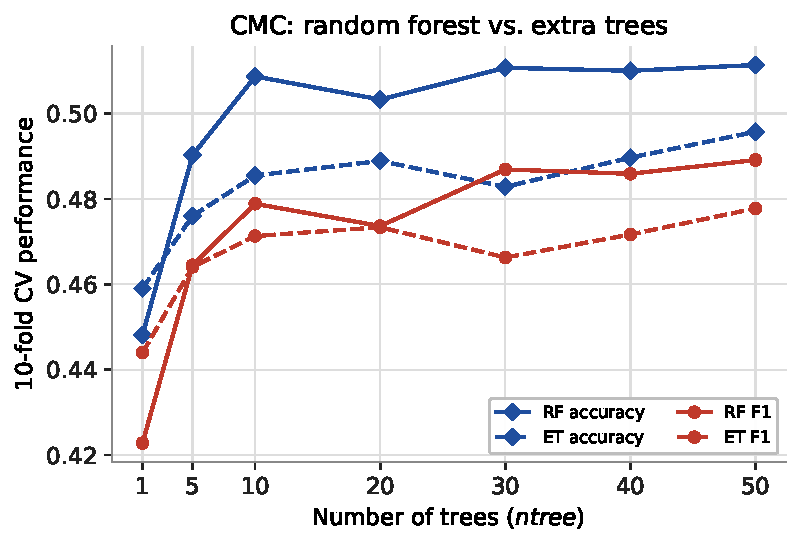
\includegraphics[width=\textwidth]{figures/cmc_et.pdf}\end{subfigure}
\caption{Random forest (solid) vs.\ extra trees (dashed), accuracy and F1 vs.\ $ntree$, each with its own best stopping criterion.}
\end{figure}

\begin{itemize}
\item \textbf{All-numerical datasets: extra trees win.} Digits goes from 0.9771 to 0.9832 and Parkinsons from 0.9031
to 0.9383, and extra trees are ahead at almost every $ntree$. With only numerical attributes, every split uses the
random threshold, so the trees disagree more and the vote averages out more of the variance. Skipping the bootstrap
matters too: on Parkinsons, with only 175 training recordings, every tree keeps all recordings of each person instead
of losing about 37\%.
\item \textbf{Rice: a tie} (0.9283 vs.\ 0.9302), within the fold-to-fold noise. All methods hit the same ceiling there.
\item \textbf{Mixed datasets: the forest wins} (Credit 0.8697 vs.\ 0.8605, CMC 0.5114 vs.\ 0.4957). Most attributes are
categorical, which are split the same way in both, so the random thresholds only change the few numerical attributes.
Without the bootstrap the trees are then more alike, and the vote helps less.
\item \textbf{Training time:} extra trees were not faster in our code (e.g.\ 17.0 vs.\ 12.9 seconds for 50 trees on
Digits). Their usual speed advantage is over searching every possible threshold, but our HW3 forest already uses the
cheap mean. The random cuts are weaker, so the trees grow deeper and have more nodes.
\end{itemize}

\end{document}
